\documentclass[11pt]{report}
\usepackage{graphicx}
\usepackage{wrapfig}
\usepackage{hyperref}
\usepackage{amsmath}
\usepackage{amssymb}
\usepackage{mathcomp}
\usepackage[english]{babel}
\usepackage{sectsty}
\usepackage{dirtytalk}
\usepackage{listings}
\usepackage{float}
\usepackage{apacite}
\graphicspath{ {./Media/} }

\usepackage{tikz}
\usetikzlibrary{automata,positioning}
\usepackage{pgfplots}

\bibliographystyle{apacite}

\usepackage{amsmath,amssymb,amsthm,textcomp}
\newcommand{\sfdagger}{{\sffamily\textdagger}}

\chapternumberfont{\Large}
\chaptertitlefont{\LARGE}

\usepackage[symbol]{footmisc}

\usepackage{tocstyle}
\usetocstyle{standard}
\usepackage{blindtext}

\newcommand{\Lagr}{\mathcal{L}}

\usepackage{lstautogobble}  % Fix relative indenting
\usepackage{color}          % Code coloring
\usepackage{zi4}            % Nice font

\definecolor{bluekeywords}{rgb}{0.13, 0.13, 1}
\definecolor{greencomments}{rgb}{0, 0.5, 0}
\definecolor{redstrings}{rgb}{0.9, 0, 0}
\definecolor{graynumbers}{rgb}{0.5, 0.5, 0.5}

\setlength\parindent{0pt}

\lstset{
    autogobble,
    columns=fullflexible,
    showspaces=false,
    showtabs=false,
    breaklines=true,
    showstringspaces=false,
    breakatwhitespace=true,
    escapeinside={(*@}{@*)},
    commentstyle=\color{greencomments},
    keywordstyle=\color{bluekeywords},
    stringstyle=\color{redstrings},
    numberstyle=\color{graynumbers},
    basicstyle=\ttfamily\footnotesize,
    frame=l,
    framesep=12pt,
    xleftmargin=12pt,
    tabsize=4,
    captionpos=b
}

\setcounter{secnumdepth}{0}
\makeatletter
\renewcommand\tableofcontents{
  \null\hfill\textbf{\Large\contentsname}\hfill\null\par
  \@mkboth{\MakeUppercase\contentsname}{\MakeUppercase\contentsname}
  \@starttoc{toc}
}
\makeatother

\begin{document}

\begin{titlepage}
	\centering
	{\scshape\LARGE Coursera \par}
	\vspace{6.5cm}
	{\LARGE \textbf{Notes}\par}
	{\LARGE Neural Networks and Deep Learning \par}
	\vfill
	{\Large\itshape Carlos Garc\'ia Gonz\'alez\par}
	\vspace{1cm}
	{\large Summer 2020 \par}
\end{titlepage}

\tableofcontents
\selectlanguage{english}
\newpage
\chapter{Neural Networks and Deep Learning}

\section{Introduction to Deep Learning}
\subsection{What is a Neural Network?}
The housing price prediction problem can be seen as the simplest of Neural Networks. First, lets start by assuming that the house pricing is only affected by its size.
\begin{center}
	\textit{Size x -> Neuron (does the determined function) -> Price y}
\end{center}
In this particular case, a RELU (Rectified Linear Unit) function [\ref{fig:F1}] is presented and is often seen in Neural Network examples. There can not be a house priced at \$0, hence the implementation of this type of function.
\begin{figure}
	\centering
	\begin{tikzpicture}
		\begin{axis}[
			domain=-3:5,
			]
			\addplot+[mark=none,red,domain=-3:0] {0};
			\addplot+[mark=none,red,domain=0:5] {x};
		\end{axis}
	\end{tikzpicture}
	\caption{Plot of an example RELU function} \label{fig:F1}
\end{figure}
A neural network is produced by taking many single neurons and by stacking them together. \\
Now let\'s add more variables for the same problem, the representation of the network would be similar to the following graph:
\begin{center}
	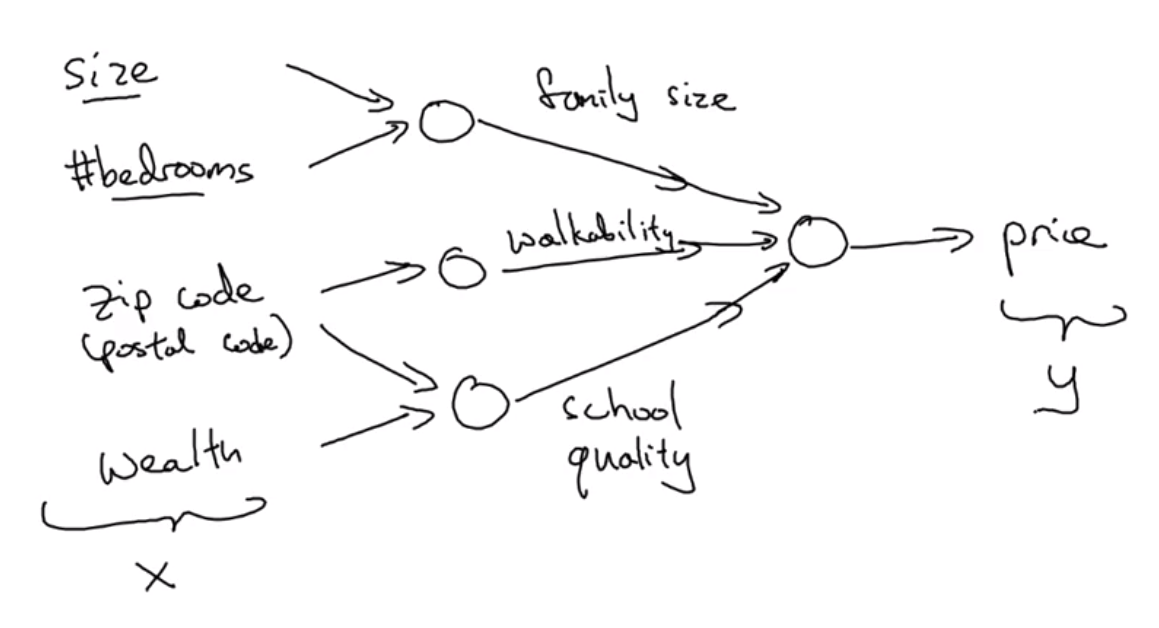
\includegraphics[width = .50\textwidth]{HPP.png}
\end{center}
The inter-connecting nods can be seen as individual RELU representations that lead to the values seen on the lines which represent important characteristics in a model and that lead to the final result; X is equal to the stack of the given inputs and Y is equal to the desired output. The \say{in-between} nods represent hidden features, these are the ones created subsequential to the input data and the network itself defines the relation between these.\\
The network processes two different types of data:
\begin{itemize}
	\item The X input values
	\item Training data
\end{itemize}
With these three the network can predict the output Y value. Giving a Neural Network enough correlational X:Y data will make it better at figuring out the sort of equations that are similar to the ones on the training data.

\subsection{Supervised Learning}
Economic value of deep learning implementations really come from Supervised learning.
You have an input x and you want to have a result y. In the previous problem it would be x = Home features, y = Price and the application would impact on the real estate business. Another example could be related to e-marketing, where x = Ad \& user info, y = Click on add? (t/f) and the would impact on online advertising. Another examples could be related to computer vision, audio recognition, machine translation and other topic related projects. Simple neural networks such as the two first examples have usually a standard NN implementation, image processing is often convolutional and sequential data implementations (such as audio, because it has a temporal component) are often recursive NN; for particular or more complex implementations there can be custom or hybrid architectures.
\begin{center}
	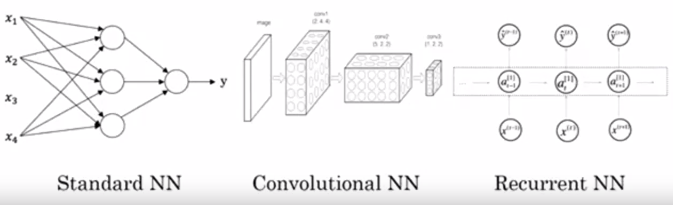
\includegraphics[width = .50\textwidth]{NNE.png}
\end{center}
Structured data (DB with specific fields) vs unstructured data (audio, images, [···]), this tangible difference is important to take into account because historically it has been more difficult to calculate from the latter, hence the importance of the architecture design importance. Although the most \say{exciting} implementations are often the unstructured data related systems, the market has more demand for well-built structured data solutions.

\subsection{Why is Deep Learning taking off?}
In the traditional learning algorithms, there was a point where the increment of input data did nothing for the performance of the system. In modern problem solving we have a lot of data to handle, so the design of a system which could profit from it was considered crucial. Neural networks are capable of incrementing the system performance in a better fashion than traditional implementations. 
\begin{center}
	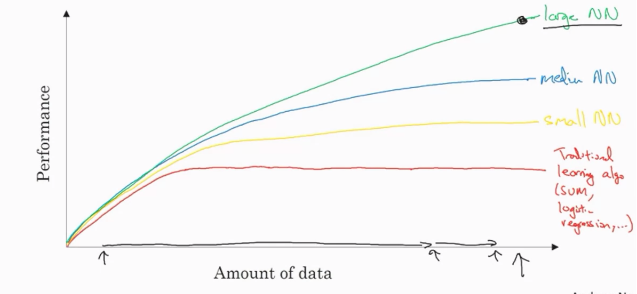
\includegraphics[width = .50\textwidth]{PRGR.png}
\end{center}
One thing to note is that the \say{Amount of Data} refers only to the amount of labeled data (contains x and y definitions). Also, the notation for the cardinality is expressed as (m).\\
Although the increment in \say{learning room} is evident, the performance also has a cap that can occur if you run out of data or if the NN is big enough that it becomes really slow to train.\\
Large neural nets are only necessary when a lot of data is required to process. There can be little to no difference in large NN and small NN systems where the data-set (m) is relatively small.\\
Deep learning progress has developed a weighted importance in data, computation-related (hardware-wise) and algorithmic advancements that allow the systems to come to a reality. One of the most notable innovations is the transition from sigmoid to RELU functions; sigmoid functions had areas (where b = 0) that led to the decrease of learning speed due to the slow parameter revision. The innovations of the three disciplines have helped the development cycle (idea -> code -> experiment) that leads to more architecture revisions.

\section{Logistic Regression as a Neural Netwoork}

\subsection{Binary Classification}
Usually the data processing is based on going through the entire dataset without explicitly using a for loop. Usually the process consists of a forward pause/forward propagation step, followed by a backward pause/backward propagation step.\\
Binary classification consists of an input x that is processed by an algorithm that outputs a binary value called label which indicates a certain input behavior or feature. For image classification (cat vs no cat), the image is decomposed to every pixel value per channel and then concatenated into a single object. \\
A single training example is denoted by the following notation:\\
$(x,y), x \in \mathbb{R}^{n_x}, y \in \{0,1\}$; where $n_x$ is the dimension of the input features x.\\
The training set is comprised of all the pairs of training examples, lowercase m is commonly used as the indicator for the number of training examples.\\
In order to put the training examples in a more compact fashion, the following model must be used:
\begin{equation}
	X =
	\begin{Bmatrix} 
	\dots & \dots & \dots & \dots\\
	x^1 & x^2 & \dots & x^m \\
	\dots & \dots & \dots & \dots\\
	\end{Bmatrix} 
 \end{equation}
This matrix $X$ will have m columns, where m is the number of training samples and $n_x$ rows ($X \in \mathbb{R}^{n_x \times m}$). Although there are other implementations, using this convention will make further implementation easier.\\
For the label output, stacking the results in columns has also been commonly used, and is defined by the following model:
\begin{equation}
	Y =
	\begin{Bmatrix} 
	y^1 & y^2 & \dots & y^m
	\end{Bmatrix}
	, Y \in \mathbb{R}^{1 \times m} 
 \end{equation}

\subsection{Logistic Regression}
Learning algorithm used when output labels Y are either 0 or 1. Given an input feature vector $x$, you need an algorithm that can output a value $\hat{y}$ representing the prediction weather the feature vector has or has not a certain behavior; the prediction of $\hat{y}$ being equal to 1 can be written as $\hat{y} = P(y=1|x)$.\\
Given the parameters $w \in \mathbb{R}^{n_x}, b \in \mathbb{R}$, we must be able to construct a function that goes through the feature vector $x$ and outputs $\hat{y}$. The function is a modification of $w^Tx + b$ so that the range does not exceed 1 or be smaller than 0, for this, the use of a sigmoid function is required. The sigmoid of $z$ [\ref{fig:F2}] can be calculated through the expression $\sigma(z)=\frac{1}{1+e^{-z}}$; if the $z$ value is very large the output will be closer to 1, on the contrary it will be closer to 0.
\begin{figure}
	\centering
	\begin{tikzpicture}
		\begin{axis}[
			domain=-3:5,
			]
            \addplot%
            [
                red,%
                mark=none,
                samples=100,
                domain=-6:6,
            ]
            (x,{1/(1+exp(-x))});
		\end{axis}
	\end{tikzpicture}
	\caption{Plot of an example sigmoid function} \label{fig:F2}
\end{figure}
Given the previous knowledge, we can now assume the following function: $z = w^Tx + b, \hat{y} = \sigma(z)$. When implementing logistic regression, it is crucial to learn parameters $w$ and $b$ so that $\hat{y}$ becomes a good estimate of the chance of $y$ being equal to 1; $b$ usually corresponds to an inter-spectrum parameter. In neural network implementations it is recommended to keep these parameters separate although there are some implementations in which these are contained in the same vector.
\newpage
\subsection{Logistic Regression Cost Function}
To train parameters $w$ and $b$ it is essential to define a cost function. As a result, it is desired that $\hat{y}^{(i)} \approx y^{(i)}$, each training example can be represented as $\hat{y} = \sigma(w^tx^{(i)}+b)$.\\
To measure the efectiveness of the developed algorithm it is necessary to use the loss function. Square error is often used in other disciplines, but due to the nature of the network-related problems the following formula is used instead: $\mathcal{L}(\hat{y},y)= -(ylog\hat{y}+(1-y)log(1-\hat{y}))$. The desired result for $\mathcal{L}$ is for it to be as small as possible.\\
The loss function checks for every training example how it is behaving, in order to check the complete training set a cost function must be used. The cost function is defined by: $J(w,b)=\frac{1}{m}\sum_{i=1}^{m} \mathcal{L}(\hat{y}^{(i)},y^{(i)})$.

\subsection{Gradient Descent}
\begin{figure}
    \centering
    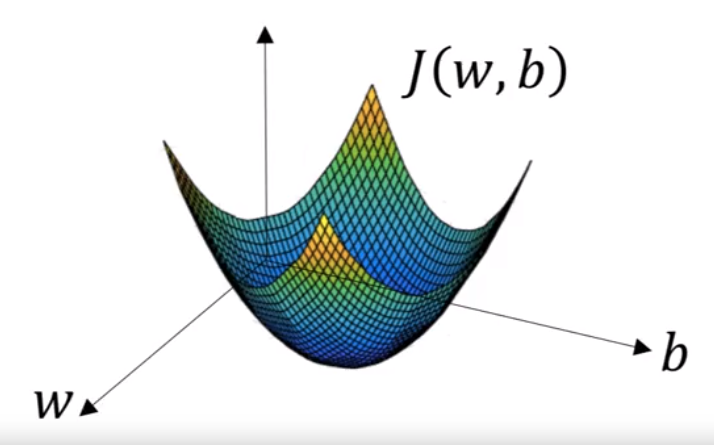
\includegraphics[width = .50\textwidth]{GD.png}
    \caption{Plot of a gradient descent} \label{fig:F3}
\end{figure}
The gradient descent algorithm is used to learn the parameters $w$ and $b$. In the figure [\ref{fig:F3}] the parameters are represented in the x and y axis while the result of the cost function $J$ is represented in the z axis. In the figure it's clear that the objective should be to find the values in which $w$ and $b$ converge while the cost function is 0. Analyzing the convex representation of the gradient descent also reveals the use of the previously-mentioned cost function; if square error was utilized, the graph would show crevices leading to erroneous calculations.\\
The process to estimate the final values consists of an \say{initial guess} for the parameters, some people use random generators for this step but is quite rare. Gradient descent starts at the given point and \say{descends} downhill through the graph until it reaches the global optimal.
\newpage
\begin{figure}
    \centering
    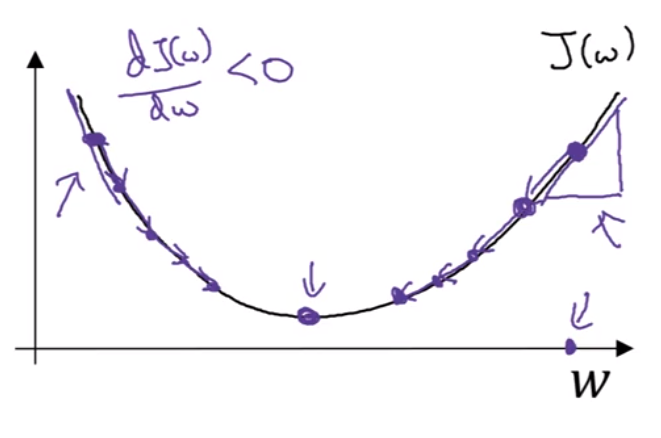
\includegraphics[width = .50\textwidth]{GDE.png}
    \caption{Example of a bidimensional gradient descent} \label{fig:F4}
\end{figure}
To better understand the gradient descent process let $J(w)$ be a concave function that we want to find the $w$ value for it to be 0; a pseudocode for the descent would be:
\begin{lstlisting}[mathescape=true]
Repeat{
    w := w - $\alpha \frac{d J(w)}{d w}$
}
\end{lstlisting}
This process is repeated until the algoritm can encounter an acceptable answer for the conversion. $\alpha$ is the representation for the learning rate, this controlls the size of the step for each iteration, and the quantity obtained by the derivative is simply the update of the change that the parameter $w$ will suffer. A visual representation can be the one on figure [\ref{fig:F4}].\\
Of course, thanks to the cost function consisting of two variables the updates would have to occur for both parameters. The updates would be the following for $J(w,b)$:\\
$w := w - \alpha \frac{\partial J(w,b)}{\partial w}, b := b - \alpha \frac{\partial J(w,b)}{\partial b}$\\

\subsection{Computation Graph}
Computation of a NNET are organized by forward pass/forward propagation in which the output is calculated, followed by a backward pass/propagation step in which the gradients are computed; the computation graph is a representation in which it's shown why it is done this way. A computation graph is a graphical representation of the calculation processes in a computer. an easy example can be the following:
\begin{center}
    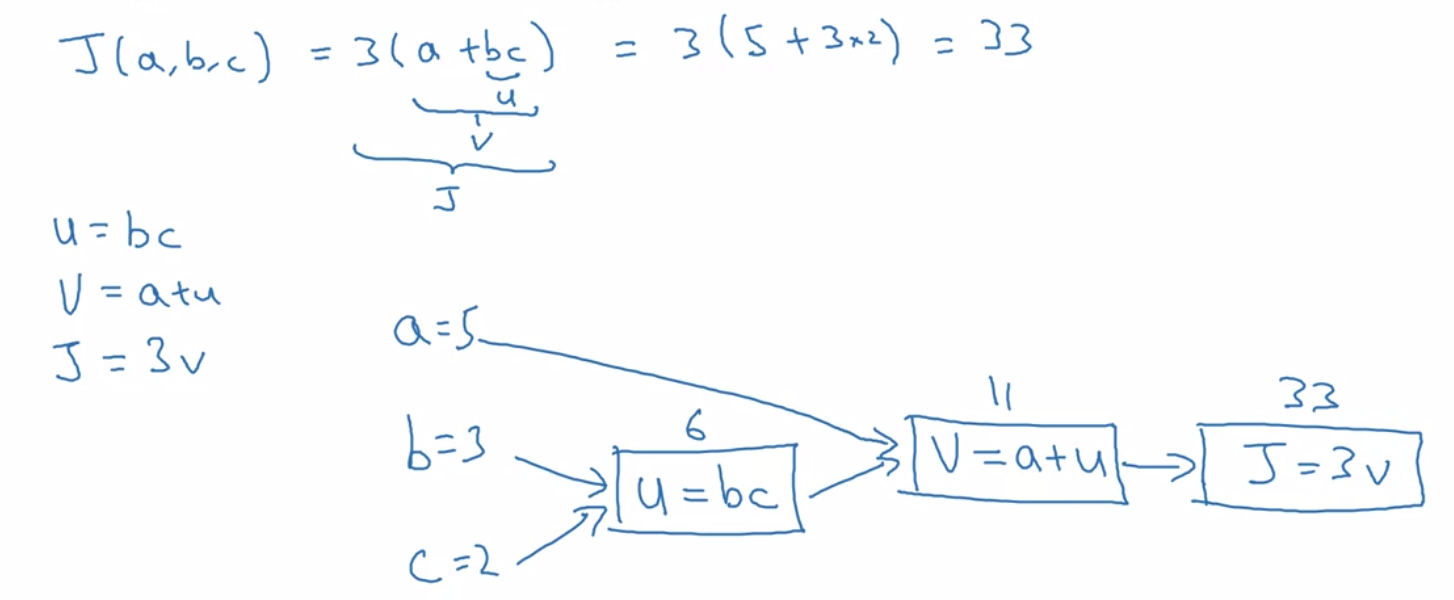
\includegraphics[width = .75\textwidth]{CG.png}
\end{center}
These are useful when there is an output variable that can be optimized; in logistic regression, the output $J$ of the cost function is expected to be minimized as much as possible. The process for this to be possible is a \say{right to left} (from the result to the original inputs) that can be translated to derivatives in computing terms.

\subsection{Derivatives with a Computation Graph}
In order to calculate the back propagation steps in the computation graphs, it is necessary to calculate multiple derivatives to show the impact of the variables in the end result. A simple example seen on the online course is the following:
\begin{center}
    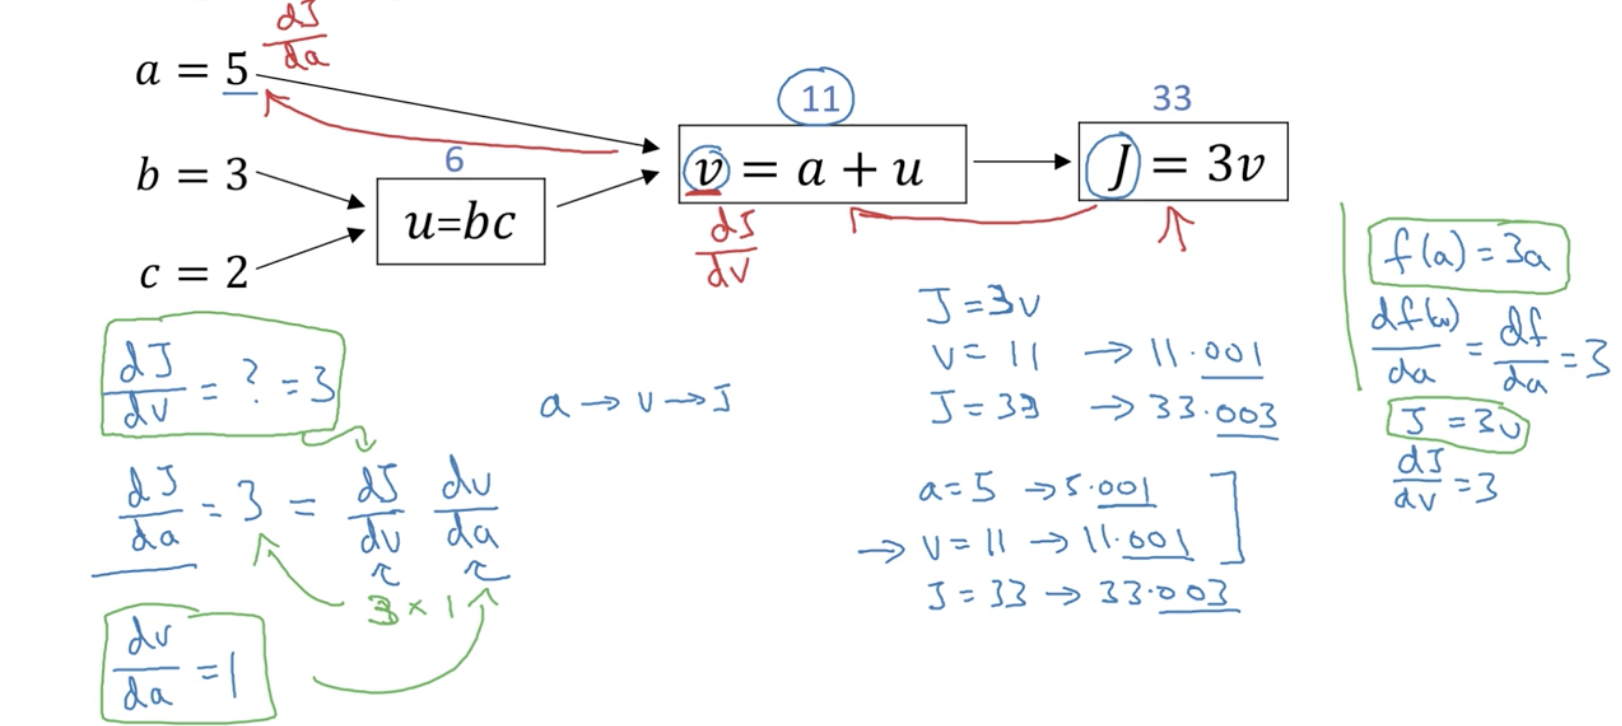
\includegraphics[width = .75\textwidth]{BPG.png}
\end{center}
For back propagation, there is usually one output variable that we care about in order to optimize it. In programming, there is a convention to write this variables so they are more understandable; in the example above this would be $J$. The calculations of the derivatives in back propagations will be this final output variable in respect of another intermediate variable of the system, and the convention follows the structure of only writing only a \say{d} followed by the index of the intermediate variable (if \say{var}, then it would be dvar).\\
\newpage
The complete example shown in the online course is the following:
\begin{center}
    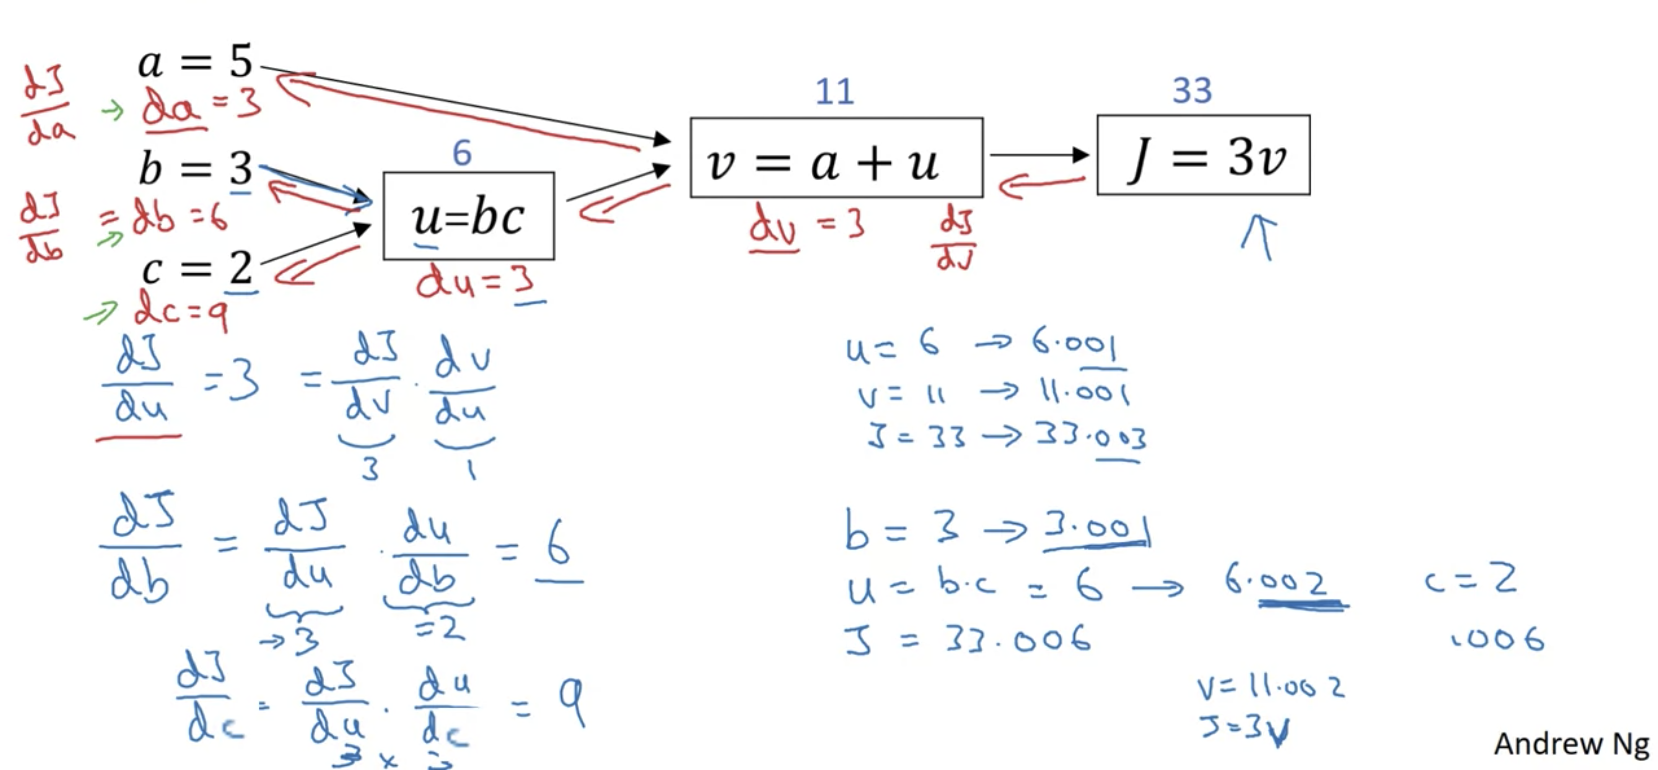
\includegraphics[width = .75\textwidth]{CBPG.png}
\end{center}
It's rather easier to compute from \say{right to left} and storing the derivatives for the chain rule as soon as the algorithm encounters its definition in order to simplify further calculations.

\subsection{Logistic Regression Gradient Descent}
Using the computation graph for gradient descent is rather overkill, but easier to begin to understand the concept. 
Recap of the functions used by the logistic regression:\\
$z = w^T    x + b\\ \hat{y} = a = \sigma(z) \\  \mathcal{L}(a,y)= -(ylog(a)+(1-y)log(1-a))$\\
The computational graph for these functions would be the following:
\begin{center}
    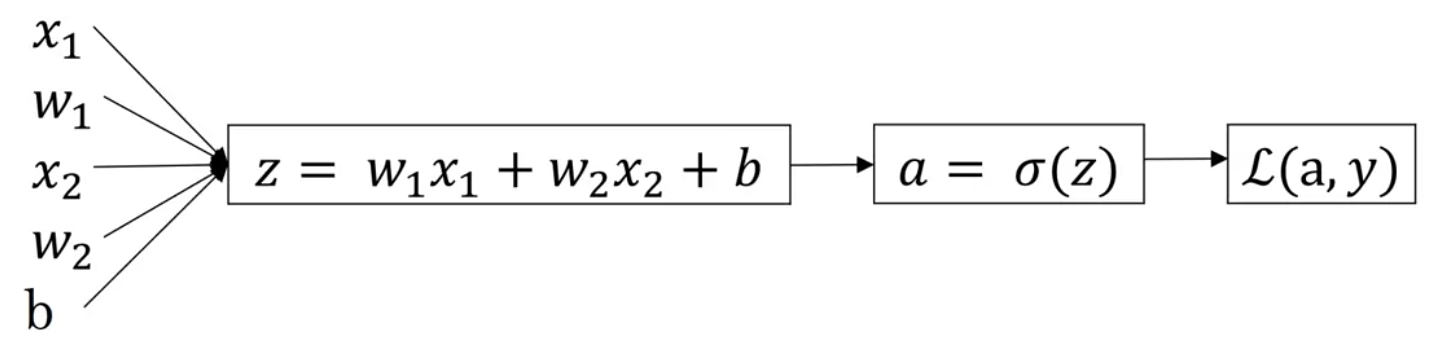
\includegraphics[width = .75\textwidth]{CGE.png}
\end{center}
In logistic regression, the goal is to modify the parameters $w_m$ and $b$ such that the funtion $\mathcal{L}$ becomes closer to 0. Using rules of derivation, we can go through the graph to calculate the derivaties:
\begin{center}
    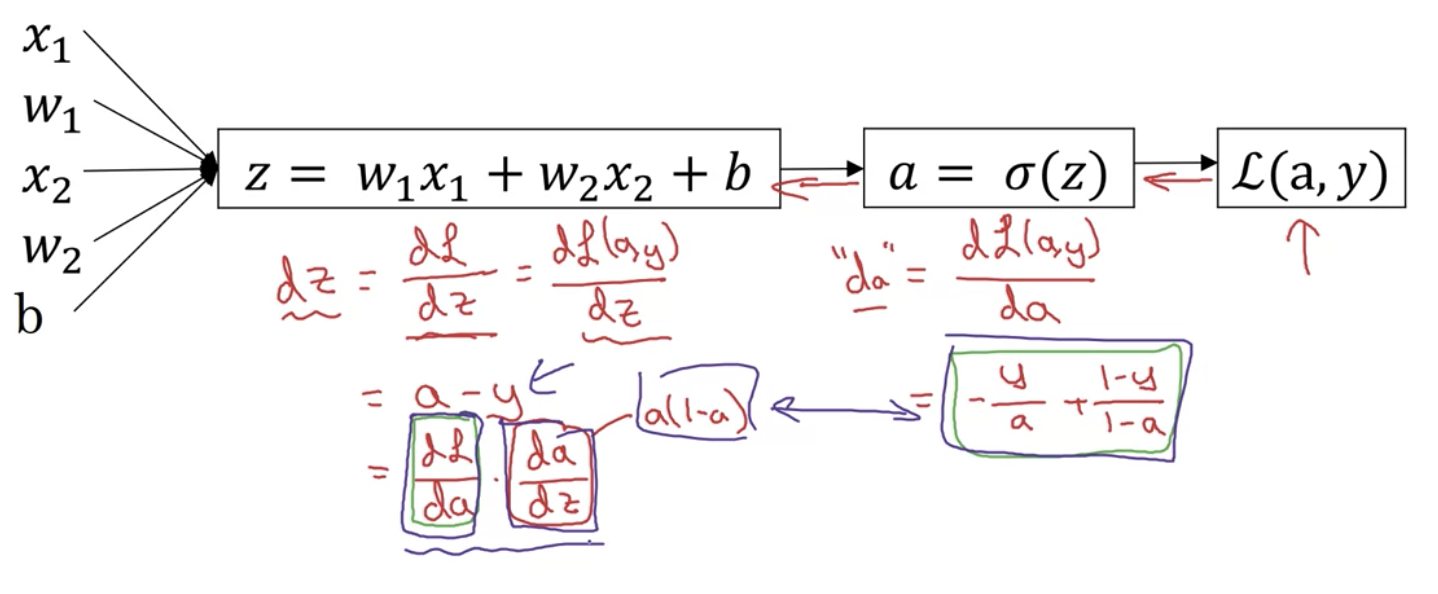
\includegraphics[width = .75\textwidth]{DCGE.png}
\end{center}
The final step for the backwards propagation process is to calculate the values for the inputs so the loss is minimal. This is calculated simply through the followinfg process: $\frac{\partial \mathcal{L}}{\partial w_{m}} = x_{m}dz $ (represented as dw\textsubscript{m} in the code), $db = dz$ and by modifying the values in the following fashion:\\
$w_m:=w_m - \alpha dw_m \\ b:= b-\alpha db$\\
It's important  to take into account that $\frac{d\mathcal{L}}{dz}=a-y$ and is represented as dz in the code.

\subsection{Gradient Descent on m Examples}
The derivative of the overall cost function in respect of a $w$ value is the average of derivatives respect to the same value of the individual loss terms, this would result in the overall gradient that will be used in gradient descent. A simple introduction to the algoritm is the following:
\begin{lstlisting}[mathescape=true]
J=0; dw$_1$=0; dw$_2$=0; db=0
For i=1 to m
    z$^{(i)}$=w$^T$x$^{(i)}$+b
    a$^{(i)}$=$\sigma$(z$^{(i)}$)
    J+=-[y$^{(i)}$log(a$^{(i)}$)+(1-y$^{(i)}$)log(1-a$^{(i)}$)]
    dz$^{(i)}$=a$^{(i)}$-y$^{(i)}$
    // This example has two training examples, if there were more they should be processed in this section 
    dw$_1$+= x$_1^{(i)}$-dz$^{(i)}$
    dw$_2$+= x$_2^{(i)}$-dz$^{(i)}$
    db+=dz$^{(i)}$
J/=m
dw$_1$/=m; dw$_2$/=m; db/=m
\end{lstlisting}
We are using the updated parameters located at the last line as accumulators, do not forget that they are the derivative of the referrenced parameter in respect of the total J function.\\
The algorithm above exemplifies only one step of the gradient descent, meaning that for it to work properly it must be repeated several times. It becomes clear that for loops could be used to solve this problem and to iterate over the w accumulators, but in deep learning algorithms explicit for loops tend to impact greatly on its efficiency. In the deep learning era it's important to avoid the use of explicit for loops to process bigger sets of data, a common solution is to use vectorization techniques.

\section{Python and Vectorization}
Vectorization is the art of removing for loops inside of the script. Deep learning nowadays is trained through big datasets, and avoiding for loops is a good practice to reduce resource cost. Where a non-vectorized algorithm goes through the whole vector iterating over the counter, vectorized scripts compute the whole vector in one step. In python, a simple script that is used to calculate z is the following:
\begin{lstlisting}[mathescape=true]
z=np.dot(w,x)+b
\end{lstlisting}
Where np is the call to the NumPy library and the dot product calculates $w^Tx$. An example was developed that showed the immense advantage of using vectorization, this can be found on the following path:
\begin{center}\texttt{0-coursera\_notes/python/1-vectorization.py}
\end{center}
It is known that GPU cores are often used in deep learning processes (although CPUs cores may also be used), these contain parallelization instructions that are called Single Instruction Multiple Data. Functions such as the np.dot() instruciton benefits greatly to the lack of explicit for loop existence and enables to take advantage of parallelization on CPUs and GPUs.\\
Using vectorization, the previously seen code for logistic regression would be something like the following pseudocode:
\begin{lstlisting}[mathescape=true]
J=0; dw=np.zeros(n-x, 1); db=0
For i=1 to m
    z$^{(i)}$=w$^T$x$^{(i)}$+b
    a$^{(i)}$=$\sigma$(z$^{(i)}$)
    J+=-[y$^{(i)}$log(a$^{(i)}$)+(1-y$^{(i)}$)log(1-a$^{(i)}$)]
    dz$^{(i)}$=a$^{(i)}$-y$^{(i)}$
    dw+=x$^{(i)}$dz$^{(i)}$
    db+=dz$^{(i)}$
J/=m
dw/=m; db/=m
\end{lstlisting}
We got rid of one for loop although there is still the one that goes through thr training examples.

\subsection{Vectorizing Logistic Regression}
To make a prediction with m training examples you have to compute the forward propagation with the following: $z^{(i)}=w^Tx^{(i)}+b$ and the activation $a=\sigma(z^{(i)})$, these for each training example. There is a way to remove the explicit for loop of the code to implement this functionality.\\
We defined $X$ as a (n$_x$, m) matrix that contains the training inputs and the objective of the vectorization process is to compute $z$ and $a$ for the whole vector in only one call inside of the code.\\
For $z$, the output matrix can be represented as a (1, m) matrix containing $[z^{(1)}, z^{(2)}, \cdots, z^{(m)}]$ and is the result of $w^TX+[b, b, \cdots, b]$ that would generate an output $[w^Tx^{(1)}+b, w^Tx^{(2)}+b, \cdots, w^Tx^{(m)}+b]$ that of course is a (1, m) vector. When you stack your training examples x horizontally it becomes $X$, and when you also stack your z values horizontally it is defined as $Z$ following the same logic. In the Python environment, the calculation for this value can be represented as:
\begin{lstlisting}[mathescape=true]
Z = np.dot(w.T,x) + b
\end{lstlisting}
Although b is a real number in this example, Python will automatically expand it as a row vector; this is known as \say{broadcasting}. Similar to $Z$ and $X$, when the values of a (the activation function) are stacked horizontally it is referenced as $A$. To implement the activation using vectorization there needs to be a calculated $Z$ which would be processed by a sigmoid function implementation.

\subsection{Vectorizing Logistic Regression's Gradient Output}
As it was shown before, the derivatives needed were calculated by doing m derivarives of the form $dz = dz^{(i)} = a^{(i)} - y^{(i)}$. Similar to the previously seen calculations, the (1, m) matrix generated with the results of the dz computations will be defined as $dZ$. Based on the previously-seen $A$ and $Y$ definitions, $dZ$ can be computed with these two variables. Although some for loops were succesfully evaded there is still one while iterating over the training examples and $db$.\\
The value of $db$ only changes by summing up the value of the multiple $dz$ outputs and calculating the average; it is essentialy $db = \frac{1}{m}\sum ^m _{i=1} dz^{(i)}$, and in Python this can be translated as:
\begin{lstlisting}[mathescape=true]
(np.sum(dZ)) / m
\end{lstlisting}
Following the same logic, $dw$ can be seen as $dw = \frac{1}{m} X dZ^T$ that in Python would look like:
\begin{lstlisting}[mathescape=true]
(X*dZ)/m
\end{lstlisting}
With these implementations, both $dw$ and $db$ are updated without the need of a single for loop. The vectorized implemenation as a whole would look something like the following pseudocode:
\begin{lstlisting}[mathescape=true]
Z = w$^T$X + b // np.dot(w.T, x) + b
A = $\sigma$(Z)
dZ = A - Y
dw = $\frac{1}{m}$ X dZ$^T$
db = $\frac{1}{m}$ np.sum(dZ)
w := w - $\alpha$ dw
b := b - $\alpha$ db
\end{lstlisting}
With this code, the forward propagation, back propagation, prediction computing and derivative computing can be processed for the m training examples withou t using a for loop. This is basically a single step for gradient descent, for it to calculate multiple steps there should be a for loop over this process for it to be possible, this should be the only for loop allowed at the moment.

\subsection{Broadcasting in Python}
The example for the following image can be located at: 
\begin{center}\texttt{0-coursera\_notes/python/2-Broadcasting.py}
\end{center}
\begin{center}
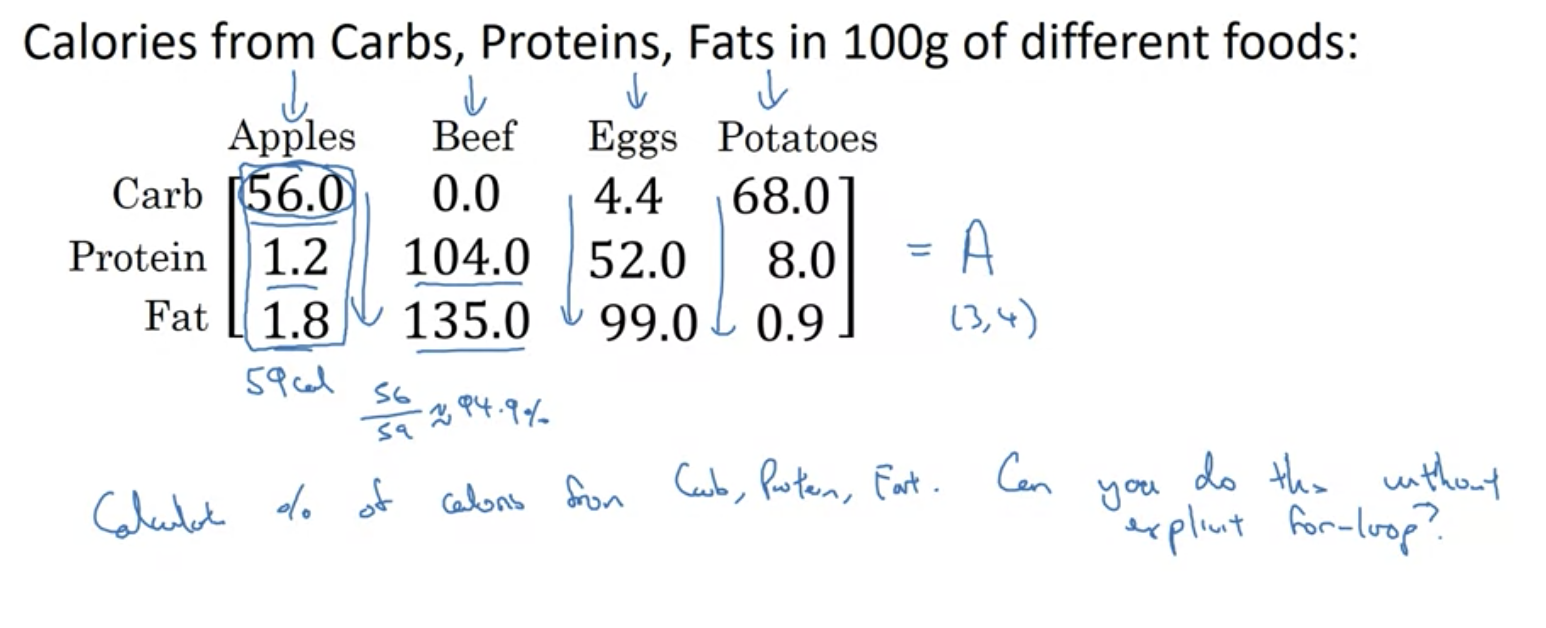
\includegraphics[width=0.9\linewidth]{Broadcast.png} 
\end{center}
In python a simple broadcast works by expanding values to fit into equations, such as the following examples:\\
\begin{equation*}
    \begin{bmatrix}
        1\\2\\3\\4
    \end{bmatrix}
    + 100 = 
    \begin{bmatrix}
        1\\2\\3\\4
    \end{bmatrix}
  + 
    \begin{bmatrix}
        100\\100\\100\\100
    \end{bmatrix}
\end{equation*}

\begin{equation*}
    \begin{bmatrix}
        1 & 2 & 3\\4 & 5 & 6
    \end{bmatrix}
    +
    \begin{bmatrix}
        100 & 200 & 300
    \end{bmatrix} =
    \begin{bmatrix}
        1 & 2 & 3\\4 & 5 & 6
    \end{bmatrix}+
    \begin{bmatrix}
        100 & 200 & 300\\100 & 200 & 300
    \end{bmatrix}
\end{equation*}
The general principle for broadcasting in python is that if you have a (m,n) matrix and you add/subtract/divide/multiply a (1,n) or (m,1) matrix it will multiply m or n times the second one and do the operation.\\
Broadcasting can be seen either as a strength or a weakness. Due to the simplicity of its implementation, there can be many errors that can be difficult to detect due to its logical nature.\\
A common error is that there can be Rank-1 arrays that have a (m,\_) dimension, calculations such as transpose would result in erroneous calculations. It is recommended in NNETs to not use data structures with the dimension in the example above. It's recommended to generate the values as column or row vectors for consistent behavior.\\
A recommendarion is to throw assertion statements around that can verify the nature of a vector, it also has documentation purposes. If a Rank-1 array is needed, the reshape function can also be used.

\subsection{Row Normalization}
Another common technique we use in Machine Learning and Deep Learning is to normalize our data. It often leads to a better performance because gradient descent converges faster after normalization. Here, by normalization we mean changing x to $ \frac{x}{\| x\|} $ (dividing each row vector of x by its norm).

\chapter{Improving Deep Neural Networks}

\chapter{Structure of Machine Learning Project}

\chapter{Convolutional Neural Networks}

\chapter{Natural Language Processing}

\chapter{Heroes of Deep Learning}
Additional to the couse's materials, there were multiple encounters with some of the most famous deep learning \say{heroes} that have a great influence in today's world. The notes below are for em to remember these scientists and some of their work.

\section{Geoffrey Hinton}
\begin{wrapfigure}{l}{0.25\textwidth}
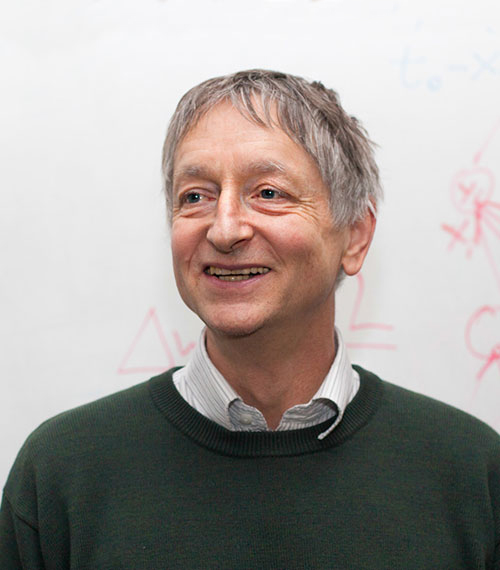
\includegraphics[width=0.9\linewidth]{GeoffH.jpeg} 
\end{wrapfigure}
Known as \textit{The Godfather of Deeplearning}, Geoffrey was inspired by indulging in how the brain stored memories. After attempting to understand it by studying it through fisiological, psychological and philosophical fields, he found it lacking a complete explanation.\\
After some time he studied AI in Edinburgh where he studied Langer Higgin's theses on neural networks which he found really interesting. While in Great Brittain he had a lot of trouble finding a job, in Califormia he encountered more openminded scientists that were interested in NNETs.\\
Although it's common belief that him and David Rumelhart invented the back propagation algorithm in 1982, many other scientists had already developed their own implementation but were not recognised as much. This paper combined two completely different strands on how the functionality of the brain which made it rater interesting. Stuart Sunderland was particularilly impressed because the back propagation algorithm had the capability of generating feature vectors from information; this was rather usefull because with the output features, it could generate new information (with the graph you can get a feature vector, and with this same vector you could derive new consistent graph-like structures). One of the most impressive examples consisted of an english text as an input that led to the generation of english words.\\
His proudest creation was the Boltzmann machine with Terry Sejnowski, these were discovered by improving an algorithm on big density connected NNETs where only few nodes could be seen and its purpose would be to discover the hidden nodes bu forward and backward passes. Further, in 2007, he found out that the features obtained by using Boltzmann machines could be used as input data, so this hidden layer could help discover the others effectively. UY Tay discovered that by combining Boltzmann machines and using sigmoid belief nets, the process could be immensley improved in its efficiency.Also, thanks to the develpopment based on ReLUs the algorithms developed by Hinton's group became very used and are now common in everyday NNET development.\\
\textit{\say{If it turns out the back prop is a really good algorithm for doing learning. Then for sure evolution could've figured out how to implement it. I mean you have cells that could turn into either eyeballs or teeth. Now, if cells can do that, they can for sure implement backpropagation and presumably this huge selective pressure for it.}} In 1987 he had an idea that the information inside the brain is sent through a recirculation algorithm that takes an idea goes through a loop where the information stays the same as it circles around, this process was asimilated to synaptic functions inside of the brain. Some time later, neuroscientists implemented the same algorithm but the other way around (where new memory is good and old memory is bad).\\
Geoffrey Hinton has been known to come with ideas that nobody believes in, he develops papers that most of the times get rejected and does not stop until he gets a publication out. For instance, he proposed that the neurons of a hiden layer could be groupped by some criterion when commonly in NNETs the hidden neurons are contained in the same layer without relation. Hinton proposes an extra structure for the relations to be represented with capsules that contain various neurons with similar characteristics.\textit{\say{So let's suppose you want to do segmentation and you have something that might be a mouth and something else that might be a nose. And you want to know if you should put them together to make one thing. So the idea should have a capsule for a mouth that has the parameters of the mouth. And you have a capsule for a nose that has the parameters of the nose. And then to decipher whether to put them together or not, you get each of them to vote for what the parameters should be for a face.}}\\
Geoffrey mentions that unsupervised learning is crucial in the long run, but you must face reality with the technological advancements we have today (almost anyone has any idea of how to develop unsupervised systems).\\
\textit{\say{Most people say you should spend several years reading the literature and then you should start working on your own ideas. And that may be true for some researchers, but for creative researchers I think what you want to do is read a little bit of the literature. And notice something that you think everybody is doing wrong, I'm contrary in that sense. You look at it and it just doesn't feel right. And then figure out how to do it right.}}\\
\textit{\say{When you have what you think is a good idea and other people think is complete rubbish, that's the sign of a really good idea.}}\\
\textit{\say{And so I think thoughts are just these great big vectors, and that big vectors have causal powers. They cause other big vectors, and that's utterly unlike the standard AI view that thoughts are symbolic expressions. }}

\bibliography{mybib.bib}

\end{document}
